\section{Methodology}
Link iO to boolean circuit and tell what we are trying to achieve.

\subsection{Hypothesis}
Thomborson proposed a space-efficient and computationally-appropriate file format (BPW) for the evaluation of very large Boolean functions with bounded program width\cite{clark}. Gates of a circuit are represented by descriptors holding information about their type (AND, OR, $\dots$) and are sequentially encoded inside the file's body. In our experiment we generate random boolean circuits (evaluating a random boolean function) with various width $w = \{ 10^3, 10^4, 10^5, 10^6, 10^7, 10^8\}$ for a fixed circuit size $N = 10^8$. The widest circuit has depth 1. The generated circuits are represented using a simplified BPW format by storing the gate type and the input indices only and by making some assumptions about the properties of the circuit under test. In particular, we make the following assumptions about the size of the circuit's inputs and outputs as well as the manner outputs from level $L_i$ are passed to gates in level $L_{i+1}$ as inputs.
\begin{enumerate}  
\item All circuits have size $N = 10^8$
\item A circuit input array has size $w$.
\item Any given level $L$ has exactly $w$ gates.
\item Every gate has only one output.
\item A circuit output array has size $w$.
\item Any given gate from a level $L_i$ has between one and three inputs that come from level $L_{i-1}$ exclusively. We can write the following:\break $G_i = f(X)$ where $f$ is a boolean operator and $X$ is an 8-byte array of size 1, 2 or 3. 
\item The output of a gate is written inside the output array at the same index of the gate. $G_i(X) = Output$ $array[i]$.
\end{enumerate}
A circuit evaluation is sequential at both gate and layer level. A Level $L_i$ is presented with an input array of size $w$ that corresponds to the output array of level $L_{i-1}$. Gates of $L_i$ are processed in ascending order of index in the level. Every gates retrieves its relevant inputs as described by the gate descriptor. Inputs indices for a gate are randomly distributed over $[0, w-1]$. We believe that this randomness will severely affect the overall performance of the circuit for large $w$ where the entire input array cannot fit in the cache. Once a gate is processed, its output is stored in the output array at the same index as the gate. Once all the gates of level $L_i$ are processed, the execution cursor moves to level $L_{i+1}$.
\par
\begin{figure}[h]
	\center
	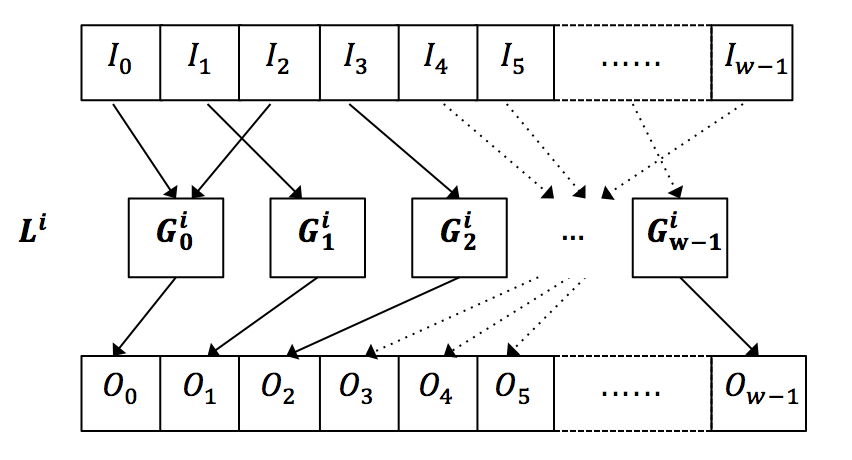
\includegraphics[width=0.8\textwidth]{img/level.png}
	\caption{Simple description of Level $L_i$ evaluation}
\end{figure}
\par
We predict that the total running time of a circuit follows this analytical model:
\begin{equation}
T = \max\{ t_g + t_e, t_m(w) \}
\end{equation}
where $T$ is the total elapsed (wallclock) time per gate, $t_g$ is the CPU time for generating a gate, $t_e$ is the CPU time for evaluating a gate, and $t_m(w)$ are the memory-stalls from the gate-generation and gate-evaluation computations.
\par
In our experiment, we generate the entire circuit prior to its evaluation. $t_g$ is in fact related to the time cost of loading of the gate for execution. We assume that this time component is near constant per gate and is not affected by the width $w$. The generation step executed initially is not monitored for performance. The resulting circuit is stacked gate by gate in a simplified BPW file. Following the initial BPW model the first 4 bytes represent the header of the a BPW file\cite{clark}. The following bytes represent the total gates of the circuit. All gates are sequentially represented from index $0$ to index $10^8-1$. A given gate's encoding varies from 9 to 25 bytes. The first byte holds the type of the gate. The following 8 to 24 bytes present the input indices encoded over 64-bits each. We could optimise the gate's representation further to compress a gate's representation but we kept this current model for simplicity. Since we fixed the size of the circuits under test to $N = 10^8$, the average size of a circuit stored in a BPW file is $avg(sizeof(Gate)) * 10^8 \approx 2 GB$ \footnote{We modelled 14 types of Gates; 1 $\times$ 1-input, 6 $\times$ 2-input and 7 $\times$ 3-input gates. On average, a gate has 2.43 inputs encoded with 8 bytes per input plus one byte for the gate type.}.
\par
We run the circuits on an x86\_64 board running Linux 3.4.6 with 16GB of \textit{RAM} and an Intel(R) Core(TM) i5-3570K CPU clocked at 3.40GHz with the following cache capacities: cache capacities: L1 = 32K for data and instructions, L2 = 256Kb and L3 = 6144Kb. Our implementation uses the \textit{unsigned long long} type to represent 8-byte variables and the \textit{char} type to represent one byte. The program is compiled using the C99 standard library.
\par
We use the \textit{perf} linux command to measure the impact of evaluating a circuit on the CPU. \textit{perf} is a tool written in C that uses Performance Counters to profile an application. Performance counters are CPU hardware registers that count hardware events such as instructions executed, cache-misses suffered, or branches mispredicted\cite{perf}. In particular, the \textit{perf stat} subcommand allows to obtain event counts that are of interest to our experiment. These events are mainly \textit{instructions, cycles} and \textit{LLC-loads}.
\par
For every value of $w$, we configure \textit{perf} to run the experiment 3 times and collect the average counts.

\par
From the results collected we established the following:

\[ T =
  \begin{cases}
    t_g + t_e       & \quad \text{if } \log_{10}(w) < 7\\
    t_m(w) & \quad \text{if } \log_{10}(w) > 7\\
  \end{cases}
\]

We estimate that $t_m(w)$ for $w = 10^3$ is negligable. In our experiment $C_{10^6}$ the total run time is assumed to reflect load and execution operations only (with no width penality) which establishes $t_g + t_e \approx 130\text{ ns}$.\footnote{ For $w = 10^3, N=10^8$, we have $N \times T = 13116 \text{ms} \implies T \approx 130 \text{ns}$ }. 
Since the CPU has a frequence of 3.40 GHz the load and execution of a gate require about 450 CPU cycles per gate\footnote{$130 \times 10^{-9} \times 3.4 \times 10^9 = 442 cycles$}, which is up to 2000 instruction per cycle (at 1.7 intruction per cycle) on a quad-core CPU assuming no stalls. For all tested $w < 10^7$ we observer a stable instruction per cycle rate at 1.7 ins/cycle with 0.2 instruction per cycle stalled.
\par
For $ w > 10^7$ the computation becomes memory-bound, allowing us to estimate $t_m(10^7) = 162$ nsec and $t_m(10^8) = 176$ nsec. Since we used 6 2-input gate types and 7 3-input gate types (out of 14 gate types), a gate evaluation will have about 2.5 memory-fetches on average to read its inputs. The gate evaluation process will also write the result in the output buffer which will cause additional memory writes. There will also be some memory-reads when reading the gate's type.
\par
Once the gate is unpacked in a top-level struct of 16 bytes (1 byte for the type, 8 bytes for the input pointer, before padding to the largest power of 2), with an average of 2.5 input indices of 8 bytes each, a level needs $ (16 + 2.5 \times 8) \times w $ of memory to be fully represented, e.g.\ levels for $w = 10^7$ need 3.6 GB. This amout of memory cannot obviously reside in cache, and on 4 GB memory plaftorms there would certainly be page-faults requiring hard disk activity. We estimate that the level array can fit inside our system's 16GB RAM without disk faults. Our initial algorithm loads an entire level before feeding it to execution loop. We could improve this by evaluating a gate as soon as it is loaded.  
\par
We designed the gate inputs to be spread randomly in an array of width $w$. For any large enough $w$, the CPU last level cache (LLC) will miss with a high probability when the input bit-array cannot be fully contained. On our test platform, LLC is 6MB wide.
\par
For w=1e5, the L3 cache occupancy of this array is still pretty high, at 1e5/6e6 = 16.6\%; so whenever a (portion of a) gate-descriptor is prefetched into a line of L3 there won't be any CPU stalls on the prefetch but there's a 16.6\% chance of evicting a line from the input array.
\par
For $w = 10^7$, the input array occupies $8 \times 10^7$ bits, the miss rate should be $1 - (6\times10^6B/10^7B) = 40\%$. From the observerd $T = 162ns$ we deduce the memory latency, which is the time required by the CPU to fetch the data from the cache, to be $162ns$ per LLC miss.\footnote{ $latency = \frac{T}{2.5 \times \text{miss rate}}$ where $T$ is the total run time per gate}. For $w = 10^8$, the expected miss rate is 94\% and the memory latency is 75ns. 




